
% Template for Elsevier CRC journal article
% version 1.1 dated 16 March 2010

% This file (c) 2010 Elsevier Ltd.  Modifications may be freely made,
% provided the edited file is saved under a different name

% This file contains modifications for Procedia Computer Science
% but may easily be adapted to other journals

% Changes since version 1.0
% - elsarticle class option changed from 1p to 3p (to better reflect CRC layout)

%-----------------------------------------------------------------------------------

%% This template uses the elsarticle.cls document class and the extension package ecrc.sty
%% For full documentation on usage of elsarticle.cls, consult the documentation "elsdoc.pdf"
%% Further resources available at http://www.elsevier.com/latex

%-----------------------------------------------------------------------------------

%%%%%%%%%%%%%%%%%%%%%%%%%%%%%%%%%%%%%%%%%%%%%%
%%%%%%%%%%%%%%%%%%%%%%%%%%%%%%%%%%%%%%%%%%%%%%
%%                                          %%
%% Important note on usage                  %%
%% -----------------------                  %%
%% This file must be compiled with PDFLaTeX %%
%% Using standard LaTeX will not work!      %%
%%                                          %%
%%%%%%%%%%%%%%%%%%%%%%%%%%%%%%%%%%%%%%%%%%%%%%
%%%%%%%%%%%%%%%%%%%%%%%%%%%%%%%%%%%%%%%%%%%%%%

%% The '3p' and 'times' class options of elsarticle are used for Elsevier CRC
\documentclass[3p,times,twocolumn]{elsarticle}

%% The `ecrc' package must be called to make the CRC functionality available
\usepackage{ecrc}
\usepackage{lipsum}

%% The ecrc package defines commands needed for running heads and logos.
%% For running heads, you can set the journal name, the volume, the starting page and the authors

%% set the volume if you know. Otherwise `00'
\volume{00}

%% set the starting page if not 1
\firstpage{1}

%% Give the name of the journal
\journalname{Software Development for Engineering Research}

%% Give the author list to appear in the running head
%% Example \runauth{C.V. Radhakrishnan et al.}
\runauth{}

%% The choice of journal logo is determined by the \jid and \jnltitlelogo commands.
%% A user-supplied logo with the name <\jid>logo.pdf will be inserted if present.
%% e.g. if \jid{yspmi} the system will look for a file yspmilogo.pdf
%% Otherwise the content of \jnltitlelogo will be set between horizontal lines as a default logo

%% Give the abbreviation of the Journal.
\jid{SDER}

%% Give a short journal name for the dummy logo (if needed)
\jnltitlelogo{}

%% Hereafter the template follows `elsarticle'.
%% For more details see the existing template files elsarticle-template-harv.tex and elsarticle-template-num.tex.

%% Elsevier CRC generally uses a numbered reference style
%% For this, the conventions of elsarticle-template-num.tex should be followed (included below)
%% If using BibTeX, use the style file elsarticle-num.bst

%% End of ecrc-specific commands
%%%%%%%%%%%%%%%%%%%%%%%%%%%%%%%%%%%%%%%%%%%%%%%%%%%%%%%%%%%%%%%%%%%%%%%%%%

%% The amssymb package provides various useful mathematical symbols
\usepackage{amssymb}
%% The amsthm package provides extended theorem environments
%% \usepackage{amsthm}

%% The lineno packages adds line numbers. Start line numbering with
%% \begin{linenumbers}, end it with \end{linenumbers}. Or switch it on
%% for the whole article with \linenumbers after \end{frontmatter}.
%% \usepackage{lineno}

%% natbib.sty is loaded by default. However, natbib options can be
%% provided with \biboptions{...} command. Following options are
%% valid:

%%   round  -  round parentheses are used (default)
%%   square -  square brackets are used   [option]
%%   curly  -  curly braces are used      {option}
%%   angle  -  angle brackets are used    <option>
%%   semicolon  -  multiple citations separated by semi-colon
%%   colon  - same as semicolon, an earlier confusion
%%   comma  -  separated by comma
%%   numbers-  selects numerical citations
%%   super  -  numerical citations as superscripts
%%   sort   -  sorts multiple citations according to order in ref. list
%%   sort&compress   -  like sort, but also compresses numerical citations
%%   compress - compresses without sorting
%%
%% \biboptions{comma,round}

% \biboptions{}

% if you have landscape tables
\usepackage[figuresright]{rotating}


\usepackage{graphicx}
\graphicspath{{./figures/}}
\DeclareGraphicsExtensions{.PNG}
% put your own definitions here:
%   \newcommand{\cZ}{\cal{Z}}
%   \newtheorem{def}{Definition}[section]
%   ...

% add words to TeX's hyphenation exception list
%\hyphenation{author another created financial paper re-commend-ed Post-Script}

% declarations for front matter

\begin{document}

\begin{frontmatter}

%% Title, authors and addresses

%% use the tnoteref command within \title for footnotes;
%% use the tnotetext command for the associated footnote;
%% use the fnref command within \author or \address for footnotes;
%% use the fntext command for the associated footnote;
%% use the corref command within \author for corresponding author footnotes;
%% use the cortext command for the associated footnote;
%% use the ead command for the email address,
%% and the form \ead[url] for the home page:
%%
%% \title{Title\tnoteref{label1}}
%% \tnotetext[label1]{}
%% \author{Name\corref{cor1}\fnref{label2}}
%% \ead{email address}
%% \ead[url]{home page}
%% \fntext[label2]{}
%% \cortext[cor1]{}
%% \address{Address\fnref{label3}}
%% \fntext[label3]{}

\dochead{}
%% Use \dochead if there is an article header, e.g. \dochead{Short communication}

\title{StoveOpt: Biomass Cookstove Optimization Tool}

%% use optional labels to link authors explicitly to addresses:
%% \author[label1,label2]{<author name>}
%% \address[label1]{<address>}
%% \address[label2]{<address>}

\author{Liam J. Cassidy}

\address{2000 SW Monroe Ave, 342 Rogers Hall, Covallis, OR 97331}
\ead{cassidyl@oregonstate.edu}


\begin{abstract}
%% Text of abstract
\end{abstract}

\begin{keyword}
%% keywords here, in the form: keyword \sep keyword

%% MSC codes here, in the form: \MSC code \sep code
%% or \MSC[2008] code \sep code (2000 is the default)

Software Development \sep%
Biomass \sep%
Cookstove \sep%
Computational Fluid Dynamics
\end{keyword}


\end{frontmatter}

%%
%% Start line numbering here if you want
%%
% \linenumbers

%% main text
\section{Introduction and Motivation}
In recent years, numerous research studies have identified a compelling case for desiging and distributing cleaner burning biomass cookstoves for low resource communities. Household air pollution, as a product of poor combustion efficiency of existing cooking technology, can cause chronic respiratory conditionsand has been linked to nearly four million premature deaths annually [REFERNCE THE CLEAN COOKING ALLIANCE PAGE--OPEN IN BROWSER]. Additionally, using biomass as a fuel source for existing inefficient cooking technology contributes significantly to global black carbon emission, which (LC PUT SOMETHING JUICY HERE FROM BOND REPORT). Identification of the pervasive lack of clean cooking technology has led to numerous investigations regarding the improvement of existing cooking technology.

Research studies in the recent past have investigated the state of clean cooking development from social, economic, and technological perspectives. BLURB ABOUT STATE OF SOCIAL. BLURB ABOUT STATE OF ECONOMICS. Within the clean cookstove industry, technical investigations focus primarily on understanding how to improve biomass combustion products and thermal efficiencies of cookstove technology.Research groups around the globe have contributed to the library of engineering evaluations of existing cookstoves by sharing model details and results of computational simulations. Many existing computational models, however, draw physical conclusions based on individual cookstove configurations leaving a vacancy in understanding for numerous different cookstove designs. The impact of producing a computational model of a biomass cookstove could be greatly improved by allowing designers to simulate a variety of cookstove configurations by way of a user-friendly open source software package.   Many (ALL MAYBE?) existing 

The intent of this paper is, first, to provide a review of existing computational modelling and software development efforts within the cookstove industry. Additionally, the paper presents version 1 (LC COME BACK HERE-is it v 1?) of the StoveOpt (LC MAKE SURE CITATIONS ARE SOLID WHEN REFERRING TO OWN SOFTWARE) software package; an open source biomass cookstove computational fluid dynamics (CFD) simulator with built in optimimzation functionality. Specifically, the paper will discuss on the methodoly used in the CFD simulations and the implementation of the software (design, layout, functionality, etc.). The paper will share results from a preliminary case, draw conclusions about the package, and establish future work.
(THIS IS KIND OF WORDY AND RUINS THE NARRATIVE--LOOK BACK HERE AND REVISE HEAVIL)


\section{Methodolgy}
%% PUT IN SUBSECTIONS FOR CFD, optimization, etc
%% In CFD discuss the models used, grid convergence (if I complete it), hardware and software used for simulations
The StoveOpt software package convert user-defined geometric parameters to create input files compatible with OpenFOAM version 6, an open-source CFD package commonly used by engineers and scientists within academia and various other industries (LIAM GO REFERENCE THE SOFTWARE FROM OPENFOAM MAIN PAGE). Analyzing results of simulations of the user-defined geometry at various secondary air flow bulk velocites automates the creation of new text based OpenFOAM input files via a simple optimization approach. Cases are created and analyzed in an iterative fashion until an optimal secondary air flow velocity is recovered from the design space. A detailed discussion of the full methodology is as follows.   

\subsection{Geometry}
The robust quality of the StoveOpt software is boasted by the abilty for a user to define any cookstove geometry, allowing for a potential interpretation and optimization of any stove design. The initial geometry definition is performed by editing a formatted Excel (REFERENCE EXCEL??) file existing within the \textit{stovegeom} folder within the StoveOpt directory. The specific parameters required to fully define the geometry are presented below in Figure 1 and Table 1 (LEE FIGURE OUT HOW TO DO FIGURES BETTER).     
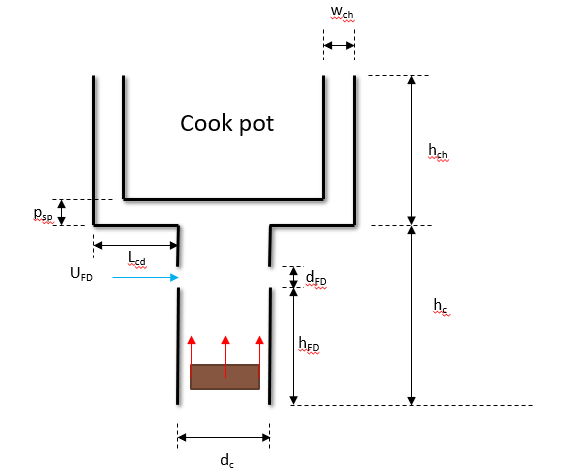
\includegraphics{geometryfrompres.PNG}

\begin{table}[h!]
	\centering
	 \begin{tabular}{||c c c c||} 
		  \hline
		   Parameter & Variable Designation \\ [0.5ex] 
		    \hline\hline
		     1 & Combustion chamber diameter & d_{c} \\ 
		      2 & Combustion chamber height & h_{c} \\
		       3 & Secondary inlet height & h_{FD} \\
			4 & Secondary inlet diameter & d_{FD} \\
			 5 & Channel width & w_{ch} \\ [1ex] 
			  6 & Channel height & h_{ch} \\ [1ex]
			   7 & Cone deck length & l_{cd} \\ [1ex]
			    8 & Pot spacing & p_[sp} \\ [1ex]
			  \hline
			   \end{tabular}
\end{table}

\subsection{Mesh}
All mesh details for OpenFOAM CFD simulations are defined in the \textit{blockMeshDict} file within the \textit{system} folder of a case directory. OpenFOAM meshes are created by defining hexehedral blocks within using vertice definitions. The StoveOpt backend uses the user-defined geometry to create within the domain. The vertices written to the \textit{blockMeshDict} file are used to create the various blocks of the cookstove model.

To validate the default level of mesh refinement, grid convergence studies are underway for the test case discussed in next sections.   (LIAM REVISIT THIS AND POTENTIALLY DO THE ACTUAL GCI)

\subsection{Physical Models}
The study calls on an existing OpenFOAM solver called \textit{reactingFoam}, a transient CFD solver that includes combustion chemisty, heat transfer for a compressible fluid flow. The various methods used to model the flow physics are as follows; note, the following information was obtained directly from the OpenFOAM API guide (v1812) (LIAM GO GET A LINK).

LIAM PUT THE GENERAL DISCRETIZED EQUATION RIGHT HERE. CAN MAKE IT GAUSS, OR VOLUMETRIC HOWEVER WANTED.

The reacting flow is assumed to be laminar throughout the computational domain. This was chosen to limit the complexity and runtime of the first attempts of the software.

The thermophysical model used to describe heat transfer due to the reaction is called \textit{psiReactionThermo}, which is a model for a reacting mixture based on the compressibility of the mixture, $\Psi$, given by:

\[$\Psi$ = (RT)^-1\] 

Where R is gas constant, and T is the temperature of the mixture. This thermophysical model serves as the basis for many of the OpenFOAM combustion solvers. The mixture is assumed to behave as an ideal gas. The transport model used is based on Sutherland's law, which computes dynamic viscosity, $\mu$, based on the absolute temperature of a mixture T, the Sutherland coefficient $A_{s}$, and Sutherland Temperature $T_{s}$. 
\[$\mu$ = (A_{s}\sqrt{T})/(1 + T_{s}/T)\]

For the purposes of this work, Sutherland coefficient and Sutherland temperature were assigned values of$1.67x10^{-6}$ and $170.67 K$ for each specie in the mixture. Specific heat capacity, $c_{p}$ was computed as a function of temperature T, based on sets of coefficients from NIST JANAF tables for each of the species included (LC REFERENCE HERE). 

\[c_{p} = R((((a_{4}T + a_{3})T + a_{2})T + a_{1})T+ a_{0})\]

Chemistry is modelled using backward (implicit) Euler method. The method was chosen to maintain stability for the stiff problem. (LC MORE DEVELOPMENT NEEDED HERE) The combustion process is assumed to be laminar for the full course of the simulation (LC MORE DEVELOPMENT NEEDED HERE).


\subsection{Temporal Schemes}
The solver uses the first order implicit Euler method for moving forward in time, 

\[(\partial(\phi))/(\partial(t)) = (\phi - \phi^{o})/(\triangle(t))\]

Where $\phi$ represents the variable from the general transport equation, $\triangle$(t) is the time time step, and $\phi^{o}$ is the general transport variable value from the previous time step.

\subsection{Spatial Schemes}

In order to approximate cell-based quantities at cell interfaces, a variety of spatial interpolation schemes were used. Gradients terms within the general transport equation were evaluated using second order central differencing (LC MAKE AN EQUATION FROM THE CFD BOOK PROBABLY). For example, the approximations for gradients of $\phi_{P}$ with neighbors $\phi_{E}$, $\phi_{W}$, $\phi_{N}$, and $\phi_{S}$ would be represented as,

\[\nabla(\phi_{P}) = (\phi_{E} - \phi_{W})/(\triangle(x)) + (\phi_{N} - \phi_{S})/(\triangle(y)\]


Where $\triangle$x and $\triangle$y are grid spacing in x-coordinate and y-coordinate directions, respectively.

Divergence terms from the general transport equation are approximated using OpenFOAM's \textit{limitedLinear}, which uses a bounded second order central differencing method (LC MIGHT NEED TO ADD MORE HERE LATER ON). 

The Laplacian terms, similar to the gradient terms, are approximated using second order central differencing of the form:

\[\nabla^{2}(\phi_{P}) = (\phi_{E}-2\phi_{P} + phi_{W})/($\triangle$x^{2}) + (\phi_{N}-2\phi_{P} + \phi_{S})/($\triangle$y^{2}$)\]

\newline

\section{Implementation}

\subsection{Software Layout}
The StoveOpt software contains a collection of modules, which are called within a the main program script. Additionally, the package contains a test suite compatible with Pytest and an input file which is to be included as a required command line argument. FIGURE XX below shows a general structure of the software package. Table XX below presents responsibilities of the modules within the package, as well the contents of the most important subdirectories (referenced from FIGURE XX) within the package..

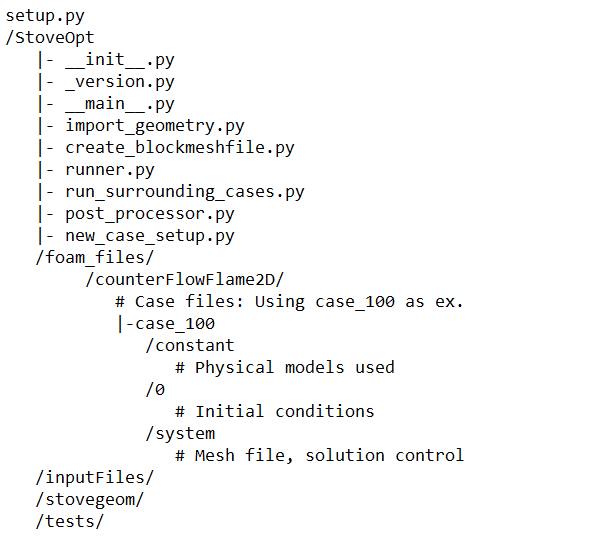
\includegraphics{skeleton.PNG}

	PUT TABLE HERE



\subsection{Functionality}



\subsection{Dependencies}
The StoveOpt software depends on various python packages, and additional software. 


\subsection{Installation}

\subsection{Running the Software}

\section{Test Case}

\section{Results}
%% Subsection for the inputs
%% subsection for results
%

\section{Conclusions}

\section{Future Work}




%% The Appendices part is started with the command \appendix;
%% appendix sections are then done as normal sections
%% \appendix

%% \section{}
%% \label{}

%% References
%%
%% Following citation commands can be used in the body text:
%% Usage of \cite is as follows:
%%   \cite{key}         ==>>  [#]
%%   \cite[chap. 2]{key} ==>> [#, chap. 2]
%%

%% References with BibTeX database:

\bibliographystyle{elsarticle-num}
\bibliography{<your-bib-database>}

%% Authors are advised to use a BibTeX database file for their reference list.
%% The provided style file elsarticle-num.bst formats references in the required Procedia style

%% For references without a BibTeX database:

% \begin{thebibliography}{00}

%% \bibitem must have the following form:
%%   \bibitem{key}...
%%

% \bibitem{}

% \end{thebibliography}

\end{document}

%%
%% End of file `ecrc-template.tex'. 
